%\documentclass[12pt]{article}

\questionheader{ex:s2.1}

%%%%%%%%%%%%%%%%%%
\subsection*{\Conceptual}
%%%%%%%%%%%%%%%%%%

%%%%%%%%%%%%%%%%%%
\begin{question}
Below is a sketch of the vector field $\vv(x,y)$. 

\[
\begin{tikzpicture}%\vv(x,y)=(x, (sinx)/(y^2+2)), -pi < x < pi
\YEaxis{5.5}{3.5}
\foreach \x in {-1,-2,-3,-4,1,2,3,4}{
\YExcoord{\x}{}
}
\foreach \x in {-1,-2,-3,1,2,3}{
\YEycoord{\x}{}
}
\foreach \x in {-4,...,4}{
\foreach \y in {-3,...,3}{
\MULTIPLY{\x}{\numberPI}{\xpi}
\DIVIDE{\xpi}{4}{\xx}
\COS{\xx}{\cosx}
\POWER{\y}{2}{\ysq}
\ADD{\ysq}{2}{\denom}
\DIVIDE{\cosx}{\denom}{\ynew}
\DIVIDE{\x}{4}{\xnew}%scale
	\draw[->, red, thick] (\x,\y)--({\x+\xnew},{\y+\ynew});
	}}
\end{tikzpicture}
\]

Find the regions where the $x$-coordinates and $y$-coordinates are positive, negative, and zero:
$\vv(x,y)\cdot \hi \begin{cases}
>0 & \mbox{ when } \fbox{\vphantom{L}\hspace{2cm}}\\
=0 &\mbox{ when } \fbox{\vphantom{L}\hspace{2cm}}\\
<0&\mbox{ when } \fbox{\vphantom{L}\hspace{2cm}}
\end{cases}$\qquad
$\vv(x,y)\cdot \hj \begin{cases}
>0 & \mbox{ when } \fbox{\vphantom{L}\hspace{2cm}}\\
=0 &\mbox{ when } \fbox{\vphantom{L}\hspace{2cm}}\\
<0&\mbox{ when } \fbox{\vphantom{L}\hspace{2cm}}
\end{cases}$

You may assume that $\vv(x,y)$ behaves as expected at the points you don't see. That is, the samples are representative of a smooth, continuous vector-valued function. You may also assume the tick marks on the axes correspond to unit distances.
\end{question}

\begin{hint} 
Not all blanks represent a single interval.
\end{hint}

\begin{answer} 
$\vv(x,y)\cdot \hi \left.\begin{cases}
>0 & \mbox{ when } \fbox{$x>0$}\\
=0 &\mbox{ when } \fbox{$x=0$}\\
<0&\mbox{ when } \fbox{$x<0$}
\end{cases}\right\}$
and
$\vv(x,y)\cdot \hj \left.\begin{cases}
>0 & \mbox{ when } \fbox{$-2<x<2$}\\
=0 &\mbox{ when } \fbox{$x \in \{-2,2\}$}\\
<0&\mbox{ when } \fbox{$x<-2$ or $x>2$}
\end{cases}\right\}$\quad
at least for $(x,y)$ shown in the sketch.
\end{answer}

\begin{solution}
The vectors are pointing to the right when $x>0$, to the left when $x<0$, and are vertical when $x=0$. So, at least for $(x,y)$ shown in the sketch,
\[\vv(x,y)\cdot \hi \begin{cases}
>0 & \mbox{ when } \fbox{$x>0$}\\
=0 &\mbox{ when } \fbox{$x=0$}\\
<0&\mbox{ when } \fbox{$x<0$}
\end{cases}\]
The behaviour of the $y$-values is more complicated. Vectors in one vertical line seem to be all pointing up, or all pointing down. So, the sign of $\vv\cdot\hj$ depends only on $x$, not on $y$ (although the \emph{magnitude} of $\vv\cdot\hj$ depends on both). Roughly,  the vectors are pointing
\begin{itemize}
\item Down when $x<-2$;
\item horizontally when $x=-2$ (remember the vector is positioned with the \emph{base} of $\vv(x,y)$ at $(x,y)$;
\item up when $-2<x<2$;
\item horizontally  when $x=2$;
\item up when $2<x$.
\end{itemize}

Since we're assuming there's nothing surprising happening between the samples pictured, at least for $(x,y)$ shown in the sketch,

\[\vv(x,y)\cdot \hj \begin{cases}
>0 & \mbox{ when } \fbox{$-2<x<2$}\\
=0 &\mbox{ when } \fbox{$x \in \{-2,2\}$}\\
<0&\mbox{ when } \fbox{$x<-2$ or $x>2$}
\end{cases}\]

\end{solution}
%%%%%%%%%%%%%%%%%%%%%%%%%%%%%%%%%%%%
\begin{question}
Below is a sketch of the vector field $\vv(x,y)$. 

\[
\begin{tikzpicture}[xscale=1.2] %\vv(x,y)=(x+y,x-y)
\YEaxis{5.5}{5.5}
\foreach \x in {-1,-2,-3,-4,1,2,3,4}{
\YExcoord{\x}{}
\YEycoord{\x}{}
}
\foreach \x in {-4,...,4}{
\foreach \y in {-4,...,4}{
\ADD{\x}{\y}{\xnew}
\SUBTRACT{\x}{\y}{\ynew}
\POWER{\x}{2}{\xtest}
\POWER{\y}{2}{\ytest}
\ADD{\xtest}{\ytest}{\test}
	\ifnum \test = 0
		{}
		\else
		\draw[->, red, thick] (\x,\y)--({\x+\xnew/6},{\y+\ynew/6});
	\fi
	}}
\draw[dotted]  (-4,-4) grid (4,4);
\end{tikzpicture}
\]

Find the regions where the $x$-coordinates and $y$-coordinates are positive, negative, and zero:

$\vv(x,y)\cdot \hi \begin{cases}
>0 & \mbox{ when } \fbox{\vphantom{L}\hspace{2cm}}\\
=0 &\mbox{ when } \fbox{\vphantom{L}\hspace{2cm}}\\
<0&\mbox{ when } \fbox{\vphantom{L}\hspace{2cm}}
\end{cases}$\qquad
$\vv(x,y)\cdot \hj \begin{cases}
>0 & \mbox{ when } \fbox{\vphantom{L}\hspace{2cm}}\\
=0 &\mbox{ when } \fbox{\vphantom{L}\hspace{2cm}}\\
<0&\mbox{ when } \fbox{\vphantom{L}\hspace{2cm}}
\end{cases}$

You may assume that the samples shown are representative of the general behaviour of $\vv(x,y)$. You may also assume the tick marks on the axes correspond to unit distances.
\end{question}

\begin{hint} 
Write down all coordinates where $\vv(x,y)\cdot\hi=0$ or $\vv(x,y)\cdot\hj=0$, and look for a pattern.
\end{hint}

\begin{answer} 
$\vv(x,y)\cdot \hi \left.\begin{cases}
>0 & \mbox{ when } \fbox{$y>-x$}\\
=0 &\mbox{ when } \fbox{$y=-x$}\\
<0&\mbox{ when } \fbox{$y<-x$}
\end{cases}\right\}$ \quad and\quad
$\vv(x,y)\cdot \hj \left.\begin{cases}
>0 & \mbox{ when } \fbox{$y<x$}\\
=0 &\mbox{ when } \fbox{$y=x$}\\
<0&\mbox{ when } \fbox{$y>x$}
\end{cases}\right\}$\quad
at least for $(x,y)$ shown in the sketch.
\end{answer}

\begin{solution}
To start out, we find the places where $\vv(x,y)\cdot\hi=0$ (vertical vectors) or $\vv(x,y)\cdot\hj=0$ (horizontal vectors). Remember the vector $\vv(x,y)$ has its \emph{tail} at $(x,y)$.

We see the vertical vectors  (those with $\vv(x,y)\cdot\hi=0$) occur at every point along the line $y=-x$, while 
horizontal vectors  (those with $\vv(x,y)\cdot\hj=0$) occur at every point along the line $y=x$.



Indeed, below the line $y=-x$, vectors point to the left, while above the line $y=-x$ they point to the right.
Similarly, vectors point down when they're above the line $y=x$, and the point up when they're below the line $y=x$.

\begin{tikzpicture}[scale=0.6] %\vv(x,y)=(x+y,x-y)
\fill[blue, opacity=0.3] (-5,5)|-(5,-5);
\draw[blue, dashed] (-5,5)--(5.5,-5.5);
\draw[blue] (-2.5,-6) node{LEFT};
\draw[red] (2.5,5.5) node{RIGHT};
\YEaxis{5.5}{5.5}
\foreach \x in {-1,-2,-3,-4,1,2,3,4}{
\YExcoord{\x}{}
\YEycoord{\x}{}
}
\foreach \x in {-4,...,4}{
\foreach \y in {-4,...,4}{
\ADD{\x}{\y}{\xnew}
\SUBTRACT{\x}{\y}{\ynew}
\POWER{\x}{2}{\xtest}
\POWER{\y}{2}{\ytest}
\ADD{\xtest}{\ytest}{\test}
	\ifnum \test = 0
		{}
		\else
		\draw[->, red, thick] (\x,\y)--({\x+\xnew/6},{\y+\ynew/6});
	\fi
	}}
\draw[dotted]  (-4,-4) grid (4,4);
\end{tikzpicture}\hfill
\begin{tikzpicture}[scale=0.6] %\vv(x,y)=(x+y,x-y)
\fill[blue, opacity=0.3] (-5,-5)-|(5,5);
\draw[blue,dashed] (-5,-5)--(5.5,5.5) ;
\draw[blue] (2.5,-6) node{UP};
\draw[red] (-2.5,5.5) node{DOWN};
\YEaxis{5.5}{5.5}
\foreach \x in {-1,-2,-3,-4,1,2,3,4}{
\YExcoord{\x}{}
\YEycoord{\x}{}
}
\foreach \x in {-4,...,4}{
\foreach \y in {-4,...,4}{
\ADD{\x}{\y}{\xnew}
\SUBTRACT{\x}{\y}{\ynew}
\POWER{\x}{2}{\xtest}
\POWER{\y}{2}{\ytest}
\ADD{\xtest}{\ytest}{\test}
	\ifnum \test = 0
		{}
		\else
		\draw[->, red, thick] (\x,\y)--({\x+\xnew/6},{\y+\ynew/6});
	\fi
	}}
\draw[dotted]  (-4,-4) grid (4,4);
\end{tikzpicture}



So, at least for $(x,y)$ shown in the sketch,
\begin{equation*}
\vv(x,y)\cdot \hi \begin{cases}
>0 & \mbox{ when } \fbox{$y>-x$}\\
=0 &\mbox{ when } \fbox{$y=-x$}\\
<0&\mbox{ when } \fbox{$y<-x$}
\end{cases} \quad \text{and} \quad
\vv(x,y)\cdot \hj \begin{cases}
>0 & \mbox{ when } \fbox{$y<x$}\\
=0 &\mbox{ when } \fbox{$y=x$}\\
<0&\mbox{ when } \fbox{$y>x$}
\end{cases}
\end{equation*}
\end{solution}

%%%%%%%%%%%%%%%%%%
\begin{question}
A platform with many small conveyor belts is aligned on a coordinate plane. Every conveyor belt moves an object on top of it in the direction of the origin, and a conveyor belt at position $(x,y)$ causes an object on top of it to move with speed $|y|$. Assume the objects do not interfere with one another.

 Give a vector-valued formula for the velocity of an object at position $(x,y)$.
 \end{question}

\begin{hint} 
If you know the speed and direction of an object, you can find its velocity.
\end{hint}

\begin{answer} 
$\vv(x,y)=\frac{-|y|}{\sqrt{x^2+y^2}}(x,y)$
\end{answer}

\begin{solution}

\item  Since all conveyors point towards the origin, the direction of motion of an object at location $(x,y)$ is $\frac{(-x,-y)}{\sqrt{x^2+y^2}}$. Its magnitude is $|y|$, so $\vv(x,y)=\frac{-|y|}{\sqrt{x^2+y^2}}(x,y)$.
\end{solution}

%%%%%%%%%%%%%%%%%%%%%%%%%%%%%%
\begin{question}
Let $\vF = P\,\hi + Q\,\hj$ be the two-dimensional vector field sketched below.
\begin{center}
      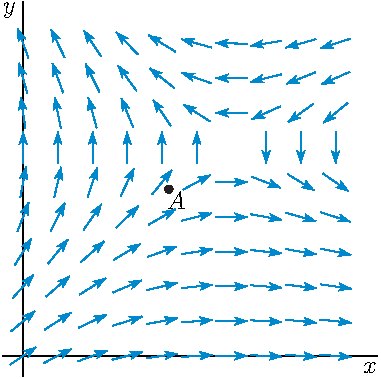
\includegraphics{VFe.pdf}
\end{center}
 Determine the signs of $P$, $Q$, $\pdiff{Q}{x}$
and $\pdiff{Q}{y}$ at the point $A$.
\end{question}

\begin{hint} 
\end{hint}

\begin{answer} 
$P>0$\qquad
$Q>0$\qquad
$\pdiff{Q}{x}<0$\qquad
$\pdiff{Q}{y}>0$
\end{answer}

\begin{solution}
The arrows near the point $A$ are pointing to the
right, indicating that $P>0$, and upward, indicating
that $Q>0$. Moving from left to right near $A$, the
vertical component of the arrows is decreasing, indicating that 
$\pdiff{Q}{x}<0$.  Moving vertically
upwards near $A$, the vertical component of the arrows is 
increasing, indicating that $\pdiff{Q}{y}>0$.

\end{solution}

%%%%%%%%%%%%%%%%%%
\begin{question}
Imagine that the vector field $\vv(x,y) = x\,\hi+y\,\hj$ 
%of part (a) of Q[\ref{prb sketch vf}] 
is the velocity field of a moving fluid.
\begin{enumerate}[(a)]
\item
At time $0$ you drop a twig into the fluid at
the point $(1,1)$. What is the approximate position of the twig
at time $t=0.01$?
\item
At time $0$ you drop a twig into the fluid at
the point $(0,0)$. What is the position of the twig
at time $t=0.01$? 
\item 
At time $0$ you drop a twig into the fluid at
the point $(0,0)$. What is the position of the twig
at time $t=10$?
\end{enumerate}
\end{question}

\begin{hint} 
When the twig is at $(x,y)$ it has velocity $\vv(x,y)$.
\end{hint}

\begin{answer} 
(a) $(1.01\,,\,1.01)$\qquad
(b) $(0\,,\,0)$\qquad
(c) $(0\,,\,0)$
\end{answer}

\begin{solution}
(a) 
At time $0$ the velocity of the twig is
$\vv(1,1) =\hi+\hj$. So at time $t=0.01$, the position of the
twig is approximately
\begin{equation*}
(1,1) + 0.01(1,1) = (1.01\,,\,1.01)
\end{equation*}

(b) 
At time $0$ the velocity of the twig is
$\vv(0,0) =\vZero$. So at time $t=0.01$, the position of the
twig is
\begin{equation*}
(0,0) + 0.01(0,0) = (0\,,\,0)
\end{equation*}

(c) At time $0$ the velocity of the twig is $\vv(0,0) =\vZero$.
So it is stationary and its velocity remains zero for all time.
The position of the twig at time $10$, and in fact at all times,
is $(0\,,\,0)$.

\end{solution}
%%%%%%%%%%%%%%%%%%

%%%%%%%%%%%%%%%%%%
\begin{question}
Imagine that the vector field $\vv(x,y) = 2x\,\hi -\hj$ 
%of part (b) of Q[\ref{prb sketch vf}] 
is the velocity field of a moving fluid.
At time $0$ you drop a twig into the fluid at
the point $(0,0)$. What is the position of the twig
at time $t=10$?
\end{question}

\begin{hint} 
Whenever the twig is on the $y$-axis, its velocity is parallel to the $y$-axis.
So it remains on the $y$-axis for all time.
\end{hint}

\begin{answer} 
$(0\,,\,-10)$
\end{answer}

\begin{solution}
The velocity of the fluid at all points of the $y$-axis
is $-\hj$. So the twig will remain on the $y$-axis and will
consequently have velocity $-\hj$ for all time. The position
of the twig at time $10$ will be
\begin{equation*}
(0,0)+10(0,-1) = (0\,,\,-10)
\end{equation*}
\end{solution}


%%%%%%%%%%%%%%%%%%
\subsection*{\Procedural}
%%%%%%%%%%%%%%%%%%


%%%%%%%%%%%%%%%%%%
\begin{question}
A platform with many small conveyor belts is aligned on a coordinate plane. Every conveyor belt moves an object on top of it in the direction of the origin, and a conveyor belt at position $(x,y)$ causes an object on top of it to move with speed $y$. Assume the objects do not interfere with one another.

 Give a vector-valued formula for the velocity of an object at position $(x,y)$.
 \end{question}

\begin{hint} 
If you know the speed and direction of an object, you can find its velocity.
\end{hint}

\begin{answer} 
$\vv(x,y)=\frac{-y}{\sqrt{x^2+y^2}}(x,y)$
\end{answer}

\begin{solution}

\item  Since all conveyors point towards the origin, the direction of motion of an object at location $(x,y)$ is $\frac{(-x,-y)}{\sqrt{x^2+y^2}}$. Its magnitude is $y$, so $\vv(x,y)=\frac{-y}{\sqrt{x^2+y^2}}(x,y)$.
\end{solution}

\begin{question}
Friendly bees fly towards your face from all directions. The  speed of each bee is inversely proportional to its distance from your face.  Find a vector field for the velocity of the swarm.
\end{question}

\begin{hint} 
Set your face to be at the origin, $(0,0,0)$. 

If $A$ is ``inversely proportional" to $B$, then there exists a constant $\alpha$ such that $AB=\alpha$. That way when $|B|$ goes up, $|A|$ goes down, and vice-versa.
\end{hint}

\begin{answer} 
If your face is at the origin, then $\vv(x,y,z)=-\frac{\alpha}{{x^2+y^2+z^2}}(x,y,z)$ for some positive constant $\alpha$.
\end{answer}

\begin{solution}
Set your face to be at the origin of our coordinate system, $(0,0,0)$. A bee at position $(x,y,z)$ is a distance of $\sqrt{x^2+y^2+z^2}$ from your face, heading in the direction $(-x,-y,-z)$. So, the unit vector indicating the direction of one friendly bee is $\frac{-1}{\sqrt{x^2+y^2+z^2}}(x,y,z)$. Now all we need to find is the length of this vector, i.e. the speed of the friendly bee.

The speed of the friendly bee is inversely proportional to $\sqrt{x^2+y^2+z^2}$, its distance from your face. (Bees that are farther away are buzzing towards you more excitedly.) So, speed is given by $\frac{\alpha}{\sqrt{x^2+y^2+z^2}}$ for some constant $\alpha$. 

The bee velocity has the direction of the unit vector $\frac{-1}{\sqrt{x^2+y^2+z^2}}(x,y,z)$ with length  $\frac{\alpha}{\sqrt{x^2+y^2+z^2}}$ for some positive constant $\alpha$. That is,
\[\vv(x,y,z)=-\frac{\alpha}{{x^2+y^2+z^2}}(x,y,z)\]
\end{solution}
%%%%%%%%%%%%%%%%%%

\begin{question}
Sketch the vector field 
$\vv(x,y)=(x^2,y)$.
\end{question}

\begin{hint} 
Start with the regions where $\vv(x,y)\cdot\hi$ and $\vv(x,y)\cdot\hj$ are positive and negative. As you move up/down/left/right, do the vectors get longer or shorter? More horizontal or more vertical?
\end{hint}

\begin{answer} 

\begin{center}
\begin{tikzpicture}
\YEaxis{5}{5}
\foreach \x in {-3,...,3}{\foreach \y in {-4,...,4}{
\POWER{\x}{2}{\xtmp}
\DIVIDE{\xtmp}{10}{\xtmp}%scale 
\ADD{\y}{0}{\ytmp}
\DIVIDE{\ytmp}{10}{\ytmp}%scale
%%we don't want to draw (0,0), so we test x^2+y^2=0. First we find x^2+y^2.
	\POWER{\xtmp}{2}{\xtest}
	\POWER{\ytmp}{2}{\ytest}
	\ADD{\xtest}{\ytest}{\test}
	\ifdim \test pt < 0.01 pt
	\draw[red, thick](\x,\y) --(\x+\xtmp,\y+\ytmp);
	{}
	\else
\draw[->, red, thick] (\x,\y) --(\x+\xtmp,\y+\ytmp);
	\fi
}}
\end{tikzpicture}
\end{center}
\end{answer}

\begin{solution}
Beginning as in the text, we note\\
$\vv(x,y)\cdot\hi=x^2 \begin{cases}
>0 & x \neq 0\\
=0 & x=0
\end{cases}$
\qquad and \qquad
$\vv(x,y)\cdot\hj=y \begin{cases}
>0 & y > 0\\
=0 & y=0\\
<0 & y<0
\end{cases}$ .\\
That leads to the following picture:
\begin{center}
\begin{tikzpicture}
\YEaxis{2.5}{2.5}
\foreach \x in {-1,0,1}{\foreach \y in {-1,0,1}{
\POWER{\x}{2}{\xtmp}
\DIVIDE{\xtmp}{2}{\xtmp} %scale
\ADD{\y}{0}{\ytmp}
\DIVIDE{\ytmp}{2}{\ytmp} %scale
\ifdim\xtmp pt=0pt
\else
\draw[->, blue, thick] (\x,\y) --(\x+\xtmp,\y);
\fi
\ifdim\ytmp pt=0 pt
\else
\draw[->, red, thick] (\x,\y) --(\x,\ytmp+\y);
\fi
}}
\end{tikzpicture}
\end{center}
This gives us a general idea to start with. Refining, we notice that when $x^2>|y|$, then the vector $\vv(x,y)$ will be more horizontal than vertical. As we move away from the $y$-axis in a horizontal line, the difference between $x^2$ and $|y|$ grows, so the vectors get more and more horizontal. However, for a fixed value of $x$, vectors farther from the axis will be more vertical than vectors closer to it.
\begin{center}
\begin{tikzpicture}
\YEaxis{5}{5}
\foreach \x in {-3,...,3}{\foreach \y in {-4,...,4}{
\POWER{\x}{2}{\xtmp}
\DIVIDE{\xtmp}{10}{\xtmp}%scale 
\ADD{\y}{0}{\ytmp}
\DIVIDE{\ytmp}{10}{\ytmp}%scale
%%we don't want to draw (0,0), so we test x^2+y^2=0. First we find x^2+y^2.
	\POWER{\xtmp}{2}{\xtest}
	\POWER{\ytmp}{2}{\ytest}
	\ADD{\xtest}{\ytest}{\test}
	\ifdim \test pt < 0.01 pt
	\draw[red, thick](\x,\y) --(\x+\xtmp,\y+\ytmp);
	{}
	\else
\draw[->, red, thick] (\x,\y) --(\x+\xtmp,\y+\ytmp);
	\fi
}}
\end{tikzpicture}
\end{center}
\end{solution}
%%%%%%%%%%%%%%%%%%%%%%%%%%%%%
\begin{question}
Sketch the \emph{direction} field of
$\vv(x,y) = \left( \sqrt{x^2+y^2}~,~\sqrt{(x-1)^2+(y-1)^2}\right)$.
\end{question}

\begin{hint} 
$\vv(x,y)\cdot \hi$ is the distance from $(x,y)$ to the origin, while $\vv(x,y)\cdot\hj$ is the distance from $(x,y)$ to the point $(1,1)$.
\end{hint}

\begin{answer} 

\begin{tikzpicture}
\YEaaxis{3}{5}{3}{5}
\foreach \x in {-1,-.5,0,.5,1,1.5,2}{\foreach \y in {-1,-.5,0,.5,1,1.5,2}{
\POWER{\x}{2}{\xsquared}
\POWER{\y}{2}{\ysquared}
\ADD{\xsquared}{\ysquared}{\tmp}
\SQUAREROOT{\tmp}{\xtmp}
\DIVIDE{\xtmp}{4}{\xtmp} %scale

%compute vertical
\SUBTRACT{\x}{1}{\xtmpa}
\POWER{\xtmpa}{2}{\xtmpb}
\SUBTRACT{\y}{1}{\ytmpa}
\POWER{\ytmpa}{2}{\ytmpb}
\ADD{\xtmpb}{\ytmpb}{\tmp}
\SQRT{\tmp}{\ytmp}
\DIVIDE{\ytmp}{4}{\ytmp} %scale

%%we don't want to draw (0,0), so we test x^2+y^2=0. First we find x^2+y^2.
	\POWER{\xtmp}{2}{\xtest}
	\POWER{\ytmp}{2}{\ytest}
	\ADD{\xtest}{\ytest}{\test}
	\ifdim \test pt < 0.01 pt
	{} % don't bother with zero vectors
	\else
	\SQUAREROOT{\test}{\L}
	\DIVIDE{\xtmp}{\L}{\xdir}
	\DIVIDE{\ytmp}{\L}{\ydir}
	\DIVIDE{\xdir}{2}{\xdir}%scale
	\DIVIDE{\ydir}{2}{\ydir}%scale
\draw[->, red, thick] (2*\x,2*\y) --(2*\x+\xdir,2*\y+\ydir);
	\fi

}}

\end{tikzpicture}
\end{answer}

\begin{solution}

Although ultimately we'll sketch only unit-length vectors, we can still find the direction of $\vv(x,y)$ by finding its $x$- and $y$ components.

Note $\vv(x,y)\cdot \hi$ is the distance from $(x,y)$ to the origin, while $\vv(x,y)\cdot\hj$ is the distance from $(x,y)$ to the point $(1,1)$. Both these numbers are always nonnegative. This leads to the following sketch:

\begin{center}
\begin{tikzpicture}
\YEaaxis{3}{5}{3}{5}
\foreach \x in {-1,-.5,0,.5,1,1.5,2}{\foreach \y in {-1,-.5,0,.5,1,1.5,2}{
\POWER{\x}{2}{\xsquared}
\POWER{\y}{2}{\ysquared}
\ADD{\xsquared}{\ysquared}{\tmp}
\SQUAREROOT{\tmp}{\xtmp}
\DIVIDE{\xtmp}{4}{\xtmp} %scale
%draw horizontal
\ifdim\xtmp pt=0pt
\else
\draw[->, blue, thick] (2*\x,2*\y) --(2*\x+\xtmp,2*\y);
\fi


%compute vertical
\SUBTRACT{\x}{1}{\xtmpa}
\POWER{\xtmpa}{2}{\xtmpb}
\SUBTRACT{\y}{1}{\ytmpa}
\POWER{\ytmpa}{2}{\ytmpb}
\ADD{\xtmpb}{\ytmpb}{\tmp}
\SQRT{\tmp}{\ytmp}
\DIVIDE{\ytmp}{4}{\ytmp} %scale
%draw vertical
\ifdim\ytmp pt=0 pt
\else
\draw[->, red, thick] (2*\x,2*\y) --(2*\x,\ytmp+2*\y);
\fi
}}
\end{tikzpicture}
\end{center}

When $(x,y)$ is far from the origin, its distance from $(0,0)$ is almost the same as its distance from $(1,0)$. So, we expect $\vv(x,y)$ to be approximately a scalar multiple of $(1,1)$. 

At $(0,0)$, $v(0,0)\cdot \hi=0$, so our vector is horizontal; similarly, $v(1,1)\cdot\hj=0$ so this vector is horizontal. Vectors very near to $(0,0)$ are nearly horizontal, while vectors near to $(1,1)$ are nearly vertical.



\begin{center}
\begin{tikzpicture}
\YEaaxis{3}{5}{3}{5}
\foreach \x in {-1,-.5,0,.5,1,1.5,2}{\foreach \y in {-1,-.5,0,.5,1,1.5,2}{
\POWER{\x}{2}{\xsquared}
\POWER{\y}{2}{\ysquared}
\ADD{\xsquared}{\ysquared}{\tmp}
\SQUAREROOT{\tmp}{\xtmp}
\DIVIDE{\xtmp}{4}{\xtmp} %scale

%compute vertical
\SUBTRACT{\x}{1}{\xtmpa}
\POWER{\xtmpa}{2}{\xtmpb}
\SUBTRACT{\y}{1}{\ytmpa}
\POWER{\ytmpa}{2}{\ytmpb}
\ADD{\xtmpb}{\ytmpb}{\tmp}
\SQRT{\tmp}{\ytmp}
\DIVIDE{\ytmp}{4}{\ytmp} %scale

%%we don't want to draw (0,0), so we test x^2+y^2=0. First we find x^2+y^2.
	\POWER{\xtmp}{2}{\xtest}
	\POWER{\ytmp}{2}{\ytest}
	\ADD{\xtest}{\ytest}{\test}
	\ifdim \test pt < 0.01 pt
	\draw[red, thick](2*\x,2*\y) --(2*\x+\xtmp,2*\y+\ytmp);
	{}
	\else
\draw[->, red, thick] (2*\x,2*\y) --(2*\x+\xtmp,2*\y+\ytmp);
	\fi

}}

\end{tikzpicture}
\end{center}

For the direction field, we normalize our vectors to have unit length.

\begin{center}
\begin{tikzpicture}
\YEaaxis{3}{5}{3}{5}
\foreach \x in {-1,-.5,0,.5,1,1.5,2}{\foreach \y in {-1,-.5,0,.5,1,1.5,2}{
\POWER{\x}{2}{\xsquared}
\POWER{\y}{2}{\ysquared}
\ADD{\xsquared}{\ysquared}{\tmp}
\SQUAREROOT{\tmp}{\xtmp}
\DIVIDE{\xtmp}{4}{\xtmp} %scale

%compute vertical
\SUBTRACT{\x}{1}{\xtmpa}
\POWER{\xtmpa}{2}{\xtmpb}
\SUBTRACT{\y}{1}{\ytmpa}
\POWER{\ytmpa}{2}{\ytmpb}
\ADD{\xtmpb}{\ytmpb}{\tmp}
\SQRT{\tmp}{\ytmp}
\DIVIDE{\ytmp}{4}{\ytmp} %scale

%%we don't want to draw (0,0), so we test x^2+y^2=0. First we find x^2+y^2.
	\POWER{\xtmp}{2}{\xtest}
	\POWER{\ytmp}{2}{\ytest}
	\ADD{\xtest}{\ytest}{\test}
	\ifdim \test pt < 0.01 pt
	{} % don't bother with zero vectors
	\else
	\SQUAREROOT{\test}{\L}
	\DIVIDE{\xtmp}{\L}{\xdir}
	\DIVIDE{\ytmp}{\L}{\ydir}
	\DIVIDE{\xdir}{2}{\xdir}%scale
	\DIVIDE{\ydir}{2}{\ydir}%scale
\draw[->, red, thick] (2*\x,2*\y) --(2*\x+\xdir,2*\y+\ydir);
	\fi

}}

\end{tikzpicture}
\end{center}
\end{solution}

%%%%%%%%%%%%%%%%%%%%%%%%%%%%%%%%%%%%

\begin{question}
Sketch the \emph{direction} field of
$\vv(x,y)=(x^2+xy,y^2-xy)$.
\end{question}

\begin{hint} 
Factor $x^2+xy=x(x+y)$ and $y^2-xy=y(x-y)$.
Chop the plane up into eight regions using the two coordinate axes and the lines $y=x$, $y=-x$.
\end{hint}

\begin{answer} 

\begin{tikzpicture}
\YEaxis{3.5}{3.5}
\foreach \x in {-3,-2.5,...,3.1}{
%compute \vv(x,y)
\POWER{\x}{2}{\xsq}
\foreach \y in {-3,-2.5,...,3.1}{
	\POWER{\y}{2}{\ysq}
	\MULTIPLY{\x}{\y}{\xy}
	\ADD{\xsq}{\xy}{\vx} % vx=x^2+xy
	\SUBTRACT{\ysq}{\xy}{\vy} % vx=y^2-xy
	%compute length
	\POWER{\vx}{2}{\vxsq}
	\POWER{\vy}{2}{\vysq}
	\ADD{\vxsq}{\vysq}{\L}
	\SQUAREROOT{\L}{\l}
	\MULTIPLY{\l}{2}{\l}%scale
	\ifdim \l pt = 0 pt %don't include zero vector at origin
		{}
		\else
		\DIVIDE{\vx}{\l}{\dx}
		\DIVIDE{\vy}{\l}{\dy}
		\draw[thick, red,->] (\x,\y)--(\x+\dx,\y+\dy);
	\fi
}}
\end{tikzpicture}
\end{answer}

\begin{solution}
The sign of $\vv(x,y) \cdot \hi = x(x+y)$ depends on the signs of $x$ and $x+y$. When they have the same signs, $\vv(x,y)\cdot \hi$ is positive, so $\vv(x,y)$ points to the right; when they have different signs, $\vv(x,y)$ points to the left.
\begin{center}
\begin{tikzpicture}
\draw (0,-3)--(0,3) node[above]{$y$};
\draw (-3,3)--(3,-3) node[right]{$y=-x$};
%\fill[pattern color=gray, pattern=north east lines] (-3,3)--(3,-3)|-cycle;
\fill[pattern color=gray, pattern=NE lines, hatch distance=5pt, hatch thickness=0.8pt] (-3,3)--(3,-3)|-cycle;
%\fill[pattern color=gray, pattern=horizontal lines] (0,-3) rectangle (3,3);
\fill[pattern color=gray, pattern=EW lines, hatch distance=5pt, hatch thickness=1.0pt] (0,-3) rectangle (3,3);
\draw[ultra thick, blue,->] (1,0)--(2,0);
\draw[ultra thick, blue,->] (-2,0)--(-1,0);
\draw[very thick, blue,->] (-.5,2)--(-1.5,2);
\draw[very thick, blue,<-] (.5,-2)--(1.5,-2);
\end{tikzpicture}
\end{center}

Similarly, the sign of $\vv(x,y) \cdot \hj = y(y-x)$ depends on the signs of $y$ and $y-x$.
\begin{center}
\begin{tikzpicture}
\draw (-3,0)--(3,0) node[right]{$x$};
\draw (-3,-3)--(3,3) node[right]{$y=x$};
%\fill[pattern color=gray, pattern=north west lines] (-3,-3)--(3,3)-|cycle;
\fill[pattern color=gray, pattern=NW lines, hatch distance=5pt, hatch thickness=1.0pt] (-3,-3)--(3,3)-|cycle;
%\fill[pattern color=gray, pattern=vertical lines] (-3,0) rectangle (3,3);
\fill[pattern color=gray, pattern=NS lines, hatch distance=5pt, hatch thickness=1.0pt] (-3,0) rectangle (3,3);
\draw[ultra thick, red,->] (-1,1)--(-1,2);
\draw[ultra thick, red,->] (1,-2)--(1,-1);
\draw[very thick, red,->] (2,1.5)--(2,.5);
\draw[very thick, red,->] (-2,-.5)--(-2,-1.5);
\end{tikzpicture}
\end{center}

All together:

\begin{center}
\begin{tikzpicture}
\YEaxis{3}{3}
\draw[help lines] (-3,-3)--(3,3) node[right]{$y=x$};
\draw[help lines] (-3,3)--(3,-3) node[right]{$y=-x$};

%equally spaced samples between regions
\foreach \x in {0,...,7}{
	\draw (0,0)+(45*\x+22.5:2.75cm) node[shape=circle,fill, minimum size=1mm, draw, inner sep=0](v\x){};}
\color{blue}%draw x-direction
\foreach \x in {7,0,1,3,4,5} %right arrows
	{\draw(v\x) node[right]{\Large$\rightarrow$};}
\foreach \x in {2,6} %left arrows
	{\draw(v\x) node[left]{\Large$\leftarrow$};}
\color{red}%draw y-direction
\foreach \x in {1,2,3,5,6,7} %up arrows
	{\draw(v\x) node[above]{\Large$\uparrow$};}
\foreach \x in {0,4} %down arrows
	{\draw(v\x) node[below]{\Large$\downarrow$};}
\end{tikzpicture}
\end{center}

Refining, we notice that  as we move straight up or down, $|\vv(x,y)\cdot \hi|$ has its minimum along the lines $y=-x$ and $x=0$. So, the vectors become more strongly vertical as we approach $y=-x$ and $x=0$ from above or below.

Similarly, $|\vv(x,y)\cdot \hj|$ has its minima along the lines $y=x$ and $y=0$, so the vectors become more strongly horizontal as we approach $y=x$ horizontally.

\begin{center}
\begin{tikzpicture}
\YEaxis{3.5}{3.5}
\foreach \x in {-3,-2.5,...,3.1}{
%compute \vv(x,y)
\POWER{\x}{2}{\xsq}
\foreach \y in {-3,-2.5,...,3.1}{
	\POWER{\y}{2}{\ysq}
	\MULTIPLY{\x}{\y}{\xy}
	\ADD{\xsq}{\xy}{\vx} % vx=x^2+xy
	\SUBTRACT{\ysq}{\xy}{\vy} % vx=y^2-xy
	%compute length
	\POWER{\vx}{2}{\vxsq}
	\POWER{\vy}{2}{\vysq}
	\ADD{\vxsq}{\vysq}{\L}
	\SQUAREROOT{\L}{\l}
	\MULTIPLY{\l}{2}{\l}%scale
	\ifdim \l pt = 0 pt %don't include zero vector at origin
		{}
		\else
		\DIVIDE{\vx}{\l}{\dx}
		\DIVIDE{\vy}{\l}{\dy}
		\draw[thick, red,->] (\x,\y)--(\x+\dx,\y+\dy);
	\fi
}}
\end{tikzpicture}
\end{center}
\end{solution}


%%%%%%%%%%%%%%%%%%
%%%%%%%%%%%%%%%%%%


%%%%%%%%%%%%%%%%%%
\begin{question}
Sketch the vector field $\displaystyle \vv(x,y)=\left[\frac{1/3}{\sqrt{x^2+y^2}}(x,y)+\frac{1/3}{\sqrt{(x-1)^2+y^2}}(x-1,y)\right]$.

%Sketch a vector field where there are two very different behaviours whether you are close to the origin or far from it. Something like $x+x^2 $ but more pronounced.

%\[\vv(x,y) = \left( x^2+y^2+\frac{1}{x^2+y^2}~,~\frac{\sqrt{x^2+y^2}}{x^2+y^2+1}\right)\]
%%
\end{question}

\begin{hint} 
What is the geometric interpretation of each summand?
\end{hint}

\begin{answer} 

\begin{tikzpicture}
\YEaxis{5}{5}
\draw (0,0) node[vertex]{};
\draw (1,0) node[vertex]{};

\foreach \x in {-4,-3.5,...,4}{
\foreach \y in {-4,-3.5,...,4}{
	
	\SUBTRACT{\x}{1}{\xless}
	\POWER{\xless}{2}{\xlsq}
	\POWER{\x}{2}{\xsq}
	\POWER{\y}{2}{\ysq}
	\ADD{\xsq}{\ysq}{\xy}
	\ADD{\xlsq}{\ysq}{\xly}
	

		\MULTIPLY{\xy}{\xly}{\testdomain}%%0 if function undefined; otherwise positive
		\SUBTRACT{\x}{.5}{\xtesta}
		\ABSVALUE{\xtesta}{\xtestb}
		\TRUNCATE[0]{\xtestb}{\testzero}%%0 if zero vector; otherwise positive
		\ADD{\testdomain}{\testzero}{\test}%%0 if don't draw; but rounding issues?
		\ifdim \test pt <.1 pt
		{}
		\else %otherwise, finish
		\SQRT{\xy}{\dena}
		\SQRT{\xly}{\denb}
		\DIVIDE{1}{\dena}{\ca}
		\DIVIDE{1}{\denb}{\cb}
		\ADD{\ca}{\cb}{\ymost}
		\MULTIPLY{\ymost}{\y}{\yunscaled}
		\DIVIDE{\yunscaled}{3}{\yy}
		\MULTIPLY{\ca}{\x}{\xa}
		\MULTIPLY{\cb}{\xless}{\xb}
		\ADD{\xa}{\xb}{\xunscaled}
		\DIVIDE{\xunscaled}{3}{\xx}
	
		\draw[red, ->] (\x,\y)--(\x+\xx,\y+\yy);
	\fi
}}
\end{tikzpicture}
\end{answer}

\begin{solution}

The field $\vv(x,y)$ is the sum, scaled by 1/3, of the unit vector pointing away from the origin and the unit vector pointing away from $(1,0)$. This tells us about a few regions:
\begin{itemize}
\item Along the $x$ axis between $(0,0)$ and $(1,0)$, the vectors away from these points are pointing in opposite directions (and have the same length), so they cancel each other out. That is, $v(x,0)=0$ for all $x \in (0,1)$. 
\item $v(0,0)$ and $v(1,0)$ are not defined.
\item Along the $x$-axis outside of $[0,1]$, the vector pointing away from the point $(0,0)$ is the same as the  vector pointing away from the point $(1,0)$. So, $v(x,0)=(-2/3,0)$ for $x<0$ and $v(x,0)=(2/3,0)$ for $x>1$.
\begin{center}
\begin{tikzpicture}
\YEaxis{5}{2}
\draw (0,0) node[vertex]{};
\draw (1,0) node[vertex]{};
\foreach \x in {-4,...,-1}
{\SUBTRACT{\x}{.33}{\xx}
\draw[->, thick, red] (\x,0)--(\xx,0);}
\foreach \x in {2,3,4}
{\ADD{\x}{.33}{\xx}
\draw[->, thick, red] (\x,0)--(\xx,0);}
\end{tikzpicture}
\end{center}
\item As the distance from $(x,y)$ to the origin grows, the vector pointing away from $(0,0)$ looks more and more like the vector pointing away from $(1,0)$. So, our vectors far away from the origin look like vectors of length about 2/3, pointing away from the origin.


\begin{center}
\begin{tikzpicture}
\YEaxis{5}{5}
\draw (0,0) node[vertex]{};
\draw (1,0) node[vertex]{};

\foreach \x in {-4,-3.5,...,4}{
\foreach \y in {-4,-3.5,...,4}{
	
	\SUBTRACT{\x}{1}{\xless}
	\POWER{\xless}{2}{\xlsq}
	\POWER{\x}{2}{\xsq}
	\POWER{\y}{2}{\ysq}
	\ADD{\xsq}{\ysq}{\xy}
	\ADD{\xlsq}{\ysq}{\xly}
	

		\MULTIPLY{\xy}{\xly}{\testdomain}%%0 if function undefined; otherwise positive
		\SUBTRACT{\x}{.5}{\xtesta}
		\ABSVALUE{\xtesta}{\xtestb}
		\TRUNCATE[0]{\xtestb}{\testzero}%%0 if zero vector; otherwise positive
		\ADD{\testdomain}{\testzero}{\test}%%0 if don't draw; but rounding issues?
		\ifdim \test pt <.1 pt
		{}
		\else %otherwise, finish
		\SQRT{\xy}{\dena}
		\SQRT{\xly}{\denb}
		\DIVIDE{1}{\dena}{\ca}
		\DIVIDE{1}{\denb}{\cb}
		\ADD{\ca}{\cb}{\ymost}
		\MULTIPLY{\ymost}{\y}{\yunscaled}
		\DIVIDE{\yunscaled}{3}{\yy}
		\MULTIPLY{\ca}{\x}{\xa}
		\MULTIPLY{\cb}{\xless}{\xb}
		\ADD{\xa}{\xb}{\xunscaled}
		\DIVIDE{\xunscaled}{3}{\xx}
	
		\draw[red, ->] (\x,\y)--(\x+\xx,\y+\yy);
	\fi
}}
\end{tikzpicture}
\end{center}
\end{itemize}
\end{solution}


%%%%%%%%%%%%%%%%%%%%%%%%%%%%%%
\begin{question}\label{prb sketch vf}
Sketch each of the following vector fields, by
drawing a figure like Figure \eref{CLP317}{fig:sourceField} 
in the CLP-4 text.
\begin{enumerate}[(a)]
\item
   $\vv(x,y) = x\,\hi+y\,\hj$.
\item
   $\vv(x,y) = 2x\,\hi -\hj$.
\item
   $\vv(x,y) = \frac{y\,\hi -x\,\hj}{\sqrt{x^2+y^2}}$.
\end{enumerate}
\end{question}

\begin{hint}
(a), (c) Intrepret the vector field geometrically. 
\end{hint}

\begin{answer} 
\begin{center}
      (a) \raisebox{-1.0\height}{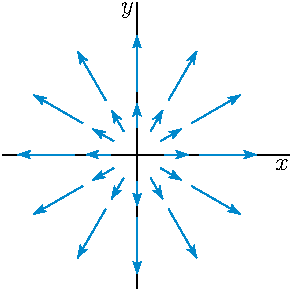
\includegraphics{VFf.pdf}}\qquad
      (b) \raisebox{-1.0\height}{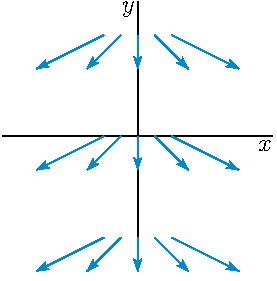
\includegraphics{VFg.pdf}}
\end{center}
\begin{center}
      (c) \raisebox{-1.0\height}{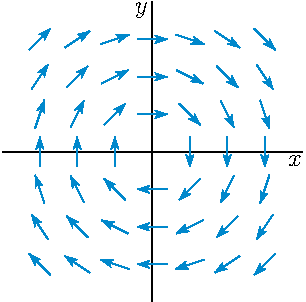
\includegraphics{VFh.pdf}}
\end{center}
\end{answer}

\begin{solution}
(a) 
The vector field $\vv(x,y) = x\,\hi+y\,\hj$ is the same as the radius
vector. It points radially outward and has length growing linearly with
the distance from the origin.
\begin{center}
      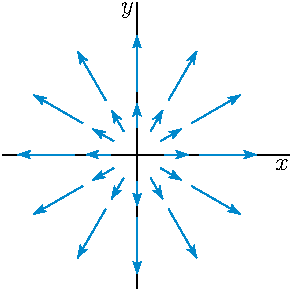
\includegraphics{VFf.pdf}
\end{center}

(b) The vertical component of  $\vv(x,y) = 2x\,\hi -\hj$
is always $-1$. Its horizontal component is $2x$, so that
\begin{itemize}\itemsep1pt \parskip0pt \parsep0pt %\itemindent-15pt
\item
$\vv(x,y)$ is rightward pointing when $x>0$
     and leftward pointing when $x<0$, and
\item
  the magnitude of the horizontal component grows
linearly with the distance from the $y$-axis. 
\end{itemize}
It is sketched in the figure on the left below.
\begin{center}
      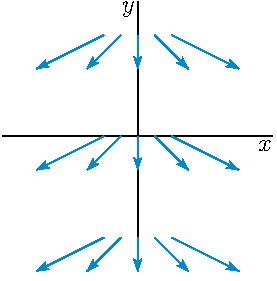
\includegraphics{VFg.pdf}\qquad
      \raisebox{-0.05\height}{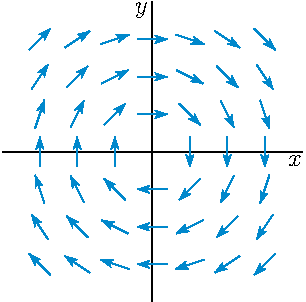
\includegraphics{VFh.pdf}}
\end{center}

(c) For every $(x,y)$ the vector 
               $\vv(x,y) = \frac{y\,\hi -x\,\hj}{\sqrt{x^2+y^2}}$
\begin{itemize}\itemsep1pt \parskip0pt \parsep0pt %\itemindent-15pt
\item
   is of length $1$ and
\item
   is perpendicular to the radius vector $x\,\hi+y\,\hj$.
\item
   $\vv(x,y)$ is rightward pointing when $y>0$
   and leftward pointing when $y<0$, and
\item
   $\vv(x,y)$ is downward pointing when $x>0$
and upward pointing when $x<0$.
\end{itemize}
It is sketched in the figure on the right above.
\end{solution}


%%%%%%%%%%%%%%%%%%
\begin{question}
A body of mass $M$ exerts a force of magnitude $\frac{GM}{D^2}$ on a particle  of unit mass distance $D$ away from itself, where $G$ is a physical constant. The force acts in the direction from the particle to the body.
\begin{center}
\begin{tikzpicture}
\draw (0,0) node[shape=circle, draw]{$M$};
\draw (2,1) node[vertex]{};
\draw[->] (2,1)--(1,.5);
\end{tikzpicture}
\end{center}

Suppose a mass of 5 kg sits at position $(0,0)$, a mass of 3 kg sits at position $(2,3)$, and a mass of 7 kg sits at position $(4,0)$ on a coordinate plane. Give the vector field $\vf(x,y)$ of the net gravitational force exerted on a unit mass at position $(x,y)$. 
\end{question}

\begin{hint} 
The constant $G$ is the same for all masses, but $M$ differs. The net force is the sum of three force vectors.
\end{hint}

\begin{answer} 
$\vf(x,y)=\frac{-5G(x,y)}{(x^2+y^2)^{3/2}}+\frac{3G(2-x,3-y)}{((x-2)^2+(y-3)^2)^{3/2}}+\frac{7G(4-x,-y)}{((x-4)^2+y^2)^{3/2}}
$
\end{answer}

\begin{solution}
A particle of unit mass at position $(x,y)$ has distance $D_1=\sqrt{x^2+y^2}$ from the 5kg mass, so that mass exerts a force of magnitude $\frac{G(5)}{x^2+y^2}$ on the particle. This force has direction $(-x,-y)$. So, the force exerted by the 5kg mass is $\vf_1(x,y)=\frac{-5G}{(x^2+y^2)^{3/2}}(x,y)$.

Similarly, the 3 kg mass at $(2,3)$ exerts a force of $\vf_2(x,y)=\frac{3G}{((x-2)^2+(y-3)^2)^{3/2}}(2-x,3-y)$; and the 7 kg mass at $(4,0)$ exerts a force of $\vf_3(x,y)=\frac{7G}{((x-4)^2+y^2)^{3/2}}(4-x,-y)$.

The net force on a unit mass is therefore
\begin{align*}
\vf(x,y)&=\vf_1(x,y)+\vf_2(x,y)+\vf_3(x,y)\\
&=\frac{-5G(x,y)}{(x^2+y^2)^{3/2}}+\frac{3G(2-x,3-y)}{((x-2)^2+(y-3)^2)^{3/2}}+\frac{7G(4-x,-y)}{((x-4)^2+y^2)^{3/2}}
\end{align*}
\end{solution}
%%%%%%%%%%%%%%%%%%

%%%%%%%%%%%%%%%%%%
\subsection*{\Application}
%%%%%%%%%%%%%%%%%%
%%%%%%%%%%%%%%%%%%
\begin{question}
\begin{enumerate}[a.]
\item 
A pole leans against a vertical wall. The pole has length 2, and it touches the wall at height $H=1$. The pole slides down, still touching the wall, with its height decreasing at a rate of $\diff{H}{t}=0.5$. 


\begin{center}
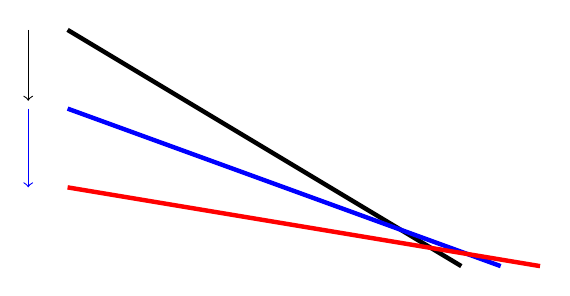
\begin{tikzpicture}
\YEaaxis{.5}{7}{.5}{3.5}
\draw[ultra thick] (5,0)--(0,3);
\draw[->] (-.5,3)--(-.5,2.1);
\color{blue}
\draw[->] (-.5,2)--(-.5,1);
\draw[ultra thick] (5.5,0)--(0,2);
\color{red}
\draw[ultra thick] (6,0)--(0,1);
\end{tikzpicture}
\end{center}
Find a vector function $\vv:\mathbb [0,2] \to \mathbb R^2$ for the velocity, when $H=1$, of a point on the pole that is $p$ units from the lower end, using the coordinate system from the sketch above. 

\item The frame of an umbrella is constructed by attaching straight, rigid poles to a common centre. The poles are all the same length, so they form radii of a circle.

The frame is lifted from the centre of the circle. The edges of the frame drag on the ground, keeping the frame in the shape of a right circular cone that is becoming taller and thinner.

\begin{center}
\begin{tikzpicture}
\draw (0,0) node[vertex]{};
\filldraw[fill opacity=0.2] (0,0)--(-2,-1) arc(180:360:2cm and .75cm)--(0,0);
\draw (0,0)--(-1,-1.65);
\draw (0,0)--(1,-1.65);
\draw[thick,->] (3,-.5)--(4,-.5);
\end{tikzpicture}
\qquad 
\begin{tikzpicture}
\draw (0,0) node[vertex]{};
\filldraw[fill opacity=0.2] (0,0)--(-1,-2) arc(180:360:1cm and .375cm)--(0,0);
\draw (0,0)--(-.5,-2.35);
\draw (0,0)--(.5,-2.35);
\end{tikzpicture}
\end{center}

Suppose the length of each pole is 2 metres, and the centre of the frame is being lifted at a rate of 50 cm/s.  Give a vector field for the velocity $\vV(x,y,z)$ of a point
           $(x,y,z)$ on the frame when its centre is 1 metre above the ground. 

Let the ground have height $z=0$, and let the centre of the frame sit directly above the origin. 
\end{enumerate}
\end{question}

\begin{hint} 
For part a., make a triangle with $P$ as one of its vertices that is similar to the triangle made by the pole, the wall, and the ground. Its hypotenuse has length $p$; let its base be $b$ and its height be $h$. Find a way to translate between $(b,h)$ and $(x,y)$.

For part b., use your answer from part a. Start by describing a point on a pole as its distance from the lower end of the pole, $p$. Then, consider $\diff{z}{t}$ and $\left(\diff{x}{t},\diff{y}{t}\right)$ separately. If you're having a hard time simplifying your answer, note  $\sqrt{x^2+y^2}=\sqrt3(1-z)$ for any point $(x,y,z)$ on a pole when $H=1$.
\end{hint}

\begin{answer} 
a. $\vv(p)=\left( \left(1-\frac{p}{2}\right)\frac{1}{2\sqrt{3}}~,~-\frac{p}{4} \right)$\qquad
b. $\vV(x,y,z)=\left(
-\frac{x}{6}, -\frac{y}{6},\frac{z}{2}\right)$ or equivalent
\end{answer}

\begin{solution}
\begin{enumerate}[a.]
\item Consider a point $P$ on the pole that is a distance $p$ away from the bottom end. Use this point to make a smaller right triangle, as in the picture below.

\begin{center}
\begin{tikzpicture}
\YEaaxis{.5}{5.5}{.5}{3.5}
\draw[thick] (5,0)-|(0,3)--cycle;
\draw (2,2) node[ above]{2};
\draw (-.5,1.5) node{$H$};
\draw (2.5,-1.25) node{$\sqrt{4-H^2}$};
\color{red}
\draw (3,1.2) node[vertex, label=above:{$P$}]{};
\filldraw[fill opacity=0.1](5,0)-|(3,1.2)--cycle;
\draw[|-|] (5.5,.5) --(3.5,1.7) node[midway, above]{$p$};
\draw (4,-.5) node{$b$};
\draw (2.5,.5) node{$h$};
\end{tikzpicture}
\end{center}

Using similar triangles:
\begin{align*}
 h&=\frac{p}{2}H  & b&=\frac{p}{2}\sqrt{4-H^2}
\intertext{If $P$ is at position $(x,y)$, then:}
 y&=h=\frac{p}{2}H & x&=\sqrt{4-H^2}-b=\left(1-\frac{p}{2}\right)\sqrt{4-H^2}\\
\diff{y}{t}&=\frac{p}{2}\diff{H}{t}=-\frac{p}{4}
&\diff{x}{t}&=\left(1-\frac{p}{2}\right)\frac{-H}{\sqrt{4-H^2}}\diff{H}{t}=\left(1-\frac{p}{2}\right)\frac{H}{2\sqrt{4-H^2}}
\intertext{When $H=1$:}
\left.\diff{y}{t}\right|_{H=1}&=-\frac{p}{4}
&\left.\diff{x}{t}\right|_{H=1}&=\left(1-\frac{p}{2}\right)\frac{1}{2\sqrt{3}}
\end{align*}
Therefore,
\[\vv(p)=\left.\left( \diff{x}{t},\diff{y}{t}\right)\right|_{H=1}=\left( \left(1-\frac{p}{2}\right)\frac{1}{2\sqrt{3}}~,~-\frac{p}{4} \right)\]

For our model, we set the domain of this function to be $[0,2]$.


\item 
Let's start by seeing what we can salvage from our work on part a.
As in part a., consider a point $P$ on one of the poles, $p$ metres from the bottom end.
\begin{center}
\begin{tikzpicture}[xscale=1.25]
\draw[thick] (5,0)-|(0,3)--cycle;
\draw (0,3) node[vertex, label=left:{$(0,0,H)$}]{};
\draw[|-|] (6,1)--(1,4) node[midway, above]{2};
\draw[|-|] (0,-.3)--(3,-.3) node[midway, below]{$\sqrt{x^2+y^2}$};
\draw[|-|] (0,-1.25)--(5,-1.25) node[midway, below]{$\sqrt{4-H^2}$};
%\draw (-.5,1.5) node{1};
\color{red}
\draw[thick, red, fill=red, fill opacity=0.1] (5,0)-|(3,1.2)--cycle;
\draw (3,1.2) node[vertex, label=left:{$P=(x,y,z)$}]{};
\draw[|-|] (5.5,.5) --(3.5,1.7) node[midway, above]{$p$};
\end{tikzpicture}
\end{center}

Let $P$ have position $(x,y,z)$. Noting that $\diff{H}{t}$ is now positive, not negative, if we stick to this two-dimensional slice,
\[ \vV(p)=\left( \left(1-\frac{p}{2}\right)\frac{-1}{2\sqrt{3}}~,~\frac{p}{4} \right) \] 
where the second coordinate is $z$ and the first coordinate refers to the (horizontal) line in the direction of the vector $(x,y,0)$.


\begin{center}
\begin{tikzpicture}[scale=2]
\draw[help lines, ->] (0,-1)--(0,1.5) node[above]{$z$};
\draw (0,1) node[vertex, label=above right:{$(0,0,H)$}]{};
\draw (0,1)--(-2,-1) arc(180:360:2cm and .75cm)--(0,1);
\filldraw[fill opacity=0.1] (0,1)--(1,-1.65)--(0,-1)--cycle;
\draw (0,-1) node[vertex, label=left:{$(0,0,0)$}]{};
\draw[->,blue] (0,-1) -- (1.5,-1.98) node[right]{$c\cdot(x,y,0)$};
\color{red}
\fill[opacity=0.2,red] (1,-1.65)--(.66,-.77)--(.66,-1.44)--cycle;
\draw[red, |-|] (.8,-.7)--(1.1,-1.6) node[midway, right]{$p$};
\draw (.66,-.77) node[vertex, label=above right:{$(x,y,z)$}]{};
\draw (.66,-1.44) node[vertex, label= left:{$(x,y,0)$}]{};
\end{tikzpicture}
\end{center}

So, we know $\displaystyle\left.\diff{z}{t}\right|_{H=1}=\frac{p}{4}$, and we know $\displaystyle\left.\left(\diff{x}{t},\diff{y}{t}\right)\right|_{H=1}=(x,y)c$ for some negative constant $c$ with $|(x,y)c|=\left(1-\frac{p}{2}\right)\frac{1}{2\sqrt{3}}$. Since we have the direction and the magnitude of the vector, we can find the vector:
\[\left.\left( \diff{x}{t},\diff{y}{t}\right)\right|_{H=1}=(x,y)c=-\frac{\left(1-\frac{p}{2}\right)}{2\sqrt 3\sqrt{x^2+y^2}}(x,y)
\]

We want our equation to be in terms of $x$, $y$, and $z$, so we need to get rid of $p$.
Using similar triangles, $\frac{p}{2}=\frac{\sqrt{4-H^2}-\sqrt{x^2+y^2}}{\sqrt{4-H^2}}$. When $H=1$, then $1-\frac{p}{2}=\frac{\sqrt{x^2+y^2}}{\sqrt3}$. So:

\[\left.\left( \diff{x}{t},\diff{y}{t}\right)\right|_{H=1}
=-\frac{1}{6}(x,y)\]

Finally:
\[\vV(x,y,z)=\left.\left( \diff{x}{t},\diff{y}{t},\diff{z}{t}\right)\right|_{H=1}=\left(
-\frac{1}{6}x~,~
-\frac{1}{6}y~,~
\frac{1}{2}z\right)\]

Not all values of $(x,y,z)$ are on the frame. But, for those values of $(x,y,z)$ that \emph{are} on the frame, this equation holds.

\end{enumerate}
\end{solution}
%%%%%%%%%%%%%%%%%%
%%%%%%%%%%%%%%%%%%
